\documentclass[aspectratio=149, xcolor=table]{beamer}
\usetheme{Montpellier}
\usefonttheme{serif}
\usecolortheme{dove}
\useinnertheme{rounded}
\setbeamersize{text margin left=5mm,text margin right=10mm}
\usefonttheme{serif}
\usepackage{graphicx}
\usepackage{babel}
\usepackage[utf8]{inputenc}
\usepackage{tabularx}
\usepackage{tikz}
\usepackage[absolute,overlay]{textpos} 
\usepackage{xcolor}
\usepackage{multicol}
\definecolor{myGreen}{RGB}{54, 114, 89}
\definecolor{unipd}{RGB}{155, 0, 20}
\definecolor{sbj1}{HTML}{77AC30}
\definecolor{sbj2}{HTML}{EDB120}
\definecolor{sbj3}{HTML}{0072BD}
\definecolor{sbj4}{HTML}{1F78B4}
\definecolor{sbj5}{HTML}{33A02C}
\definecolor{sbj6}{HTML}{E31A1C}
% Per il tema Montpellier
%\setbeamercolor{separation line}{bg=myGreen!20}
\setbeamercolor{separation line}{bg=black!20}
%\setbeamercolor{title in head/foot}{bg=white, fg=myGreen}
\setbeamercolor{title in head/foot}{bg=white, fg=black}
%\setbeamercolor{section in head/foot}{bg=white, fg=myGreen}
%\setbeamercolor{subsection in head/foot}{bg=white, fg=myGreen}
%\setbeamercolor{background canvas}{bg=white}
%\setbeamercolor{title}{fg=myGreen}
%\setbeamercolor{item}{fg =myGreen}
%\setbeamercolor{frametitle}{fg = myGreen}
%\setbeamercolor{section in toc}{fg=myGreen!80}
%\setbeamercolor{subsection in toc}{fg=black}
\setbeamerfont{section in toc}{series=\bfseries,size=\normalsize}
\setbeamerfont{frametitle}{series=\bfseries}
%\setbeamerfont{title}{family=\scshape}
%\setbeamercolor{frametitle}{fg=unipd}
%\setbeamercolor{section in head/foot}{bg=unipd, fg=white}
%\setbeamercolor{subsection in head/foot}{fg=unipd}
%\setbeamercolor{author in head/foot}{bg=unipd, fg=white}
%\setbeamercolor{title in head/foot}{fg=unipd}
%\setbeamercolor{date in head/foot}{fg=unipd}

\usepackage{tikz}
\usetikzlibrary{shapes.geometric, arrows}

\tikzstyle{startstop} = [rectangle, rounded corners, minimum width=3cm, minimum height=1cm,text centered, draw=black]
\tikzstyle{process} = [rectangle, minimum width=3cm, minimum height=1cm, text centered, draw=black]
\tikzstyle{decision} = [diamond, minimum width=1.5cm, minimum height=0.5cm, text centered, draw=black]
\tikzstyle{arrow} = [thick,->,>=stealth]

% definisce gli elementi da mettere sopra la figura 
% rectangles on figures 
\newcommand{\imagenode}[2][1]% [scale], filename
{   \node[above right,inner sep=0] (myimage) {\includegraphics[scale=#1]{#2}};
	\path (myimage.north east);
	\pgfgetlastxy{\myimagex}{\myimagey}
	\pgfmathsetmacro{\myimagewidth}{\myimagex/28.453}
	\pgfmathsetmacro{\myimageheight}{\myimagey/28.453}
}
\newcommand{\imagegrid}[4][help lines]% [options], steps, font, precision
{   \pgfkeys{/pgf/number format/.cd,fixed,precision=#4}
	\foreach \x in {0,...,#2}
	{   \draw[#1] (\x/#2*\myimagewidth,\myimageheight) -- (\x/#2*\myimagewidth,0) node[below] {#3\pgfmathparse{\x/#2}\pgfmathprintnumber{\pgfmathresult}};
		\draw[#1] (\myimagewidth,\x/#2*\myimageheight) -- (0,\x/#2*\myimageheight) node[left] {#3\pgfmathparse{\x/#2}\pgfmathprintnumber{\pgfmathresult}};
	}
}

\newcommand{\highlightbox}[8][densely dashed,thick]% [options], left, low, right, up, node options, node text, overlay spec
{   \only<#8>{\draw[#1] (#2*\myimagewidth, #3*\myimageheight) rectangle node[#6] {#7} (#4*\myimagewidth, #5*\myimageheight);}
}

\newcommand{\highlighttext}[8][densely dashed,thick]% [options], left, low, right, up, node options, node text, overlay spec
{   \only<#8>{\path[#1] (#2*\myimagewidth, #3*\myimageheight) rectangle node[#6] {#7} (#4*\myimagewidth, #5*\myimageheight);}
}

% tikz per la cfa 

\usetikzlibrary{shapes.geometric, arrows}
\tikzstyle{latent} = [ellipse, minimum width=2.5cm, minimum height=2cm,text centered, draw=black]
\tikzstyle{item} = [rectangle, rounded corners, minimum width=0.5cm, minimum height=1cm, text width =1.5cm, text centered, draw=black]
\tikzstyle{arrow} = [thick,->,>=stealth]

% allegedly, il codice che viene dopo permette di cambiare colore alle celle 

\makeatletter
\def\rowcolor{\noalign{\ifnum0=`}\fi\bmr@rowcolor}
\newcommand<>{\bmr@rowcolor}{%
	\alt#1%
	{\global\let\CT@do@color\CT@@do@color\@ifnextchar[\CT@rowa\CT@rowb}% 
	{\ifnum0=`{\fi}\@gooble@rowcolor}% 
}

\newcommand{\@gooble@rowcolor}[2][]{\@gooble@rowcolor@}
\newcommand{\@gooble@rowcolor@}[1][]{\@gooble@rowcolor@@}
\newcommand{\@gooble@rowcolor@@}[1][]{\ignorespaces}
\makeatother



\makeatletter
\def\cellcolor{{\ifnum0=`}\fi\bmr@cellcolor}
\newcommand<>{\bmr@cellcolor}{%
	\alt#1%
	{\global\let\CT@do@color\CT@@do@color\@ifnextchar[\CT@rowa\CT@rowb}% 
	{\ifnum0=`{\fi}\@gooble@cellcolor}% 
}

\newcommand{\@gooble@cellcolor}[2][]{\@gooble@cellcolor@}
\newcommand{\@gooble@cellcolor@}[1][]{\@gooble@cellcolor@@}
\newcommand{\@gooble@cellcolor@@}[1][]{\ignorespaces}
\makeatother

\DeclareMathOperator*{\argmax}{arg\,max}
\DeclareMathOperator*{\argmin}{arg\,min}

\AtBeginSection[]
{
	\begin{frame}
		\tableofcontents[currentsection, currentsubsection]
	\end{frame}
}

\AtBeginSubsection[]
{
	\begin{frame}
		\tableofcontents[currentsection, currentsubsection]
	\end{frame}
}


\title[ILA]{It's how you use the items that counts: \\ An intelligent procedure for item selection in Item Response Theory}
\titlegraphic{%
	\vspace{-3mm}
	
\includegraphics[width=1.8cm,height=1.8cm,keepaspectratio]{img/unitn.png}%\hspace*{9.75cm}~%
	
\includegraphics[width=2.5cm,height=1.8cm,keepaspectratio]{img/psicostat.jpg}%
	
\includegraphics[width=1.8cm,height=1.8cm,keepaspectratio]{img/logoUnipd.jpg}%
}

\author{ \vspace{-5mm} Ottavia M. Epifiania\textsuperscript{1,2}, Pasquale Anselmi\textsuperscript{3}, Egidio Robusto\textsuperscript{3}}


\institute [UniPd] {
	%\includegraphics[width=10mm]{unipd.png}\\ 
	\textsuperscript{1} Psychology and Cognitive Science Department, University of Trento, Italy \\
	\textsuperscript{2} Psicostat, University of Padova, Italy \\
	\textsuperscript{3} Department of Philosophy, Sociology, Education, and Applied Psychology,	University of Padova, Italy}

\date [ASA2024] {%\vspace{0.6cm}\\
	Convegno ASA 2024, Contributed session: \\ Developing, administering and refining measurement instruments in Social Sciences}
\begin{document}
\begin{frame}[plain]
    \maketitle
\end{frame}

\section{Aim}
\begin{frame}
	\small
	Item Response Theory (IRT) for the development of Short Test Form (STF):
	
	\textbf{Typical procedure:}
Manually inspecting the item characteristics to recreate the desired characteristics of a test 
	
	\onslide<2->
\textbf{\textcolor{unipd}{Issue}}
		
		Not an automated procedure $\rightarrow$ depends on the subjectivity of the researcher

	
	\onslide<1->
		\textbf{Automated (new) procedure:}
 A priori definition of latent trait levels of interest on which the STF should be focusing the most
	
	\onslide<3->
\textbf{\textcolor{unipd}{Issue}}
		
		 Punctual definition of the specific latent trait levels of interest influences the number of selected items

\onslide<4->
\begin{center}
	\color{myGreen}\textsc{AIM}
\end{center}
	
 New automated procedure for item selection in IRT that only requires the definition of the desired characteristics of a test 

\end{frame}

\section{Item Response Theory and Information Functions}
\subsection{2-Parameter Logistic Model}

\begin{frame}
\centering

	
	\centering
	\onslide<1>
	\vspace*{1mm}
	
	$P(x_{pi} = 1|\theta_p, b_i, a_i) = \frac{\exp[a_i(\theta_p - b_i)]}{1 + \exp[a_i(\theta_p - b_i)]}$
	
	\vspace{1.5mm}
	\centering
	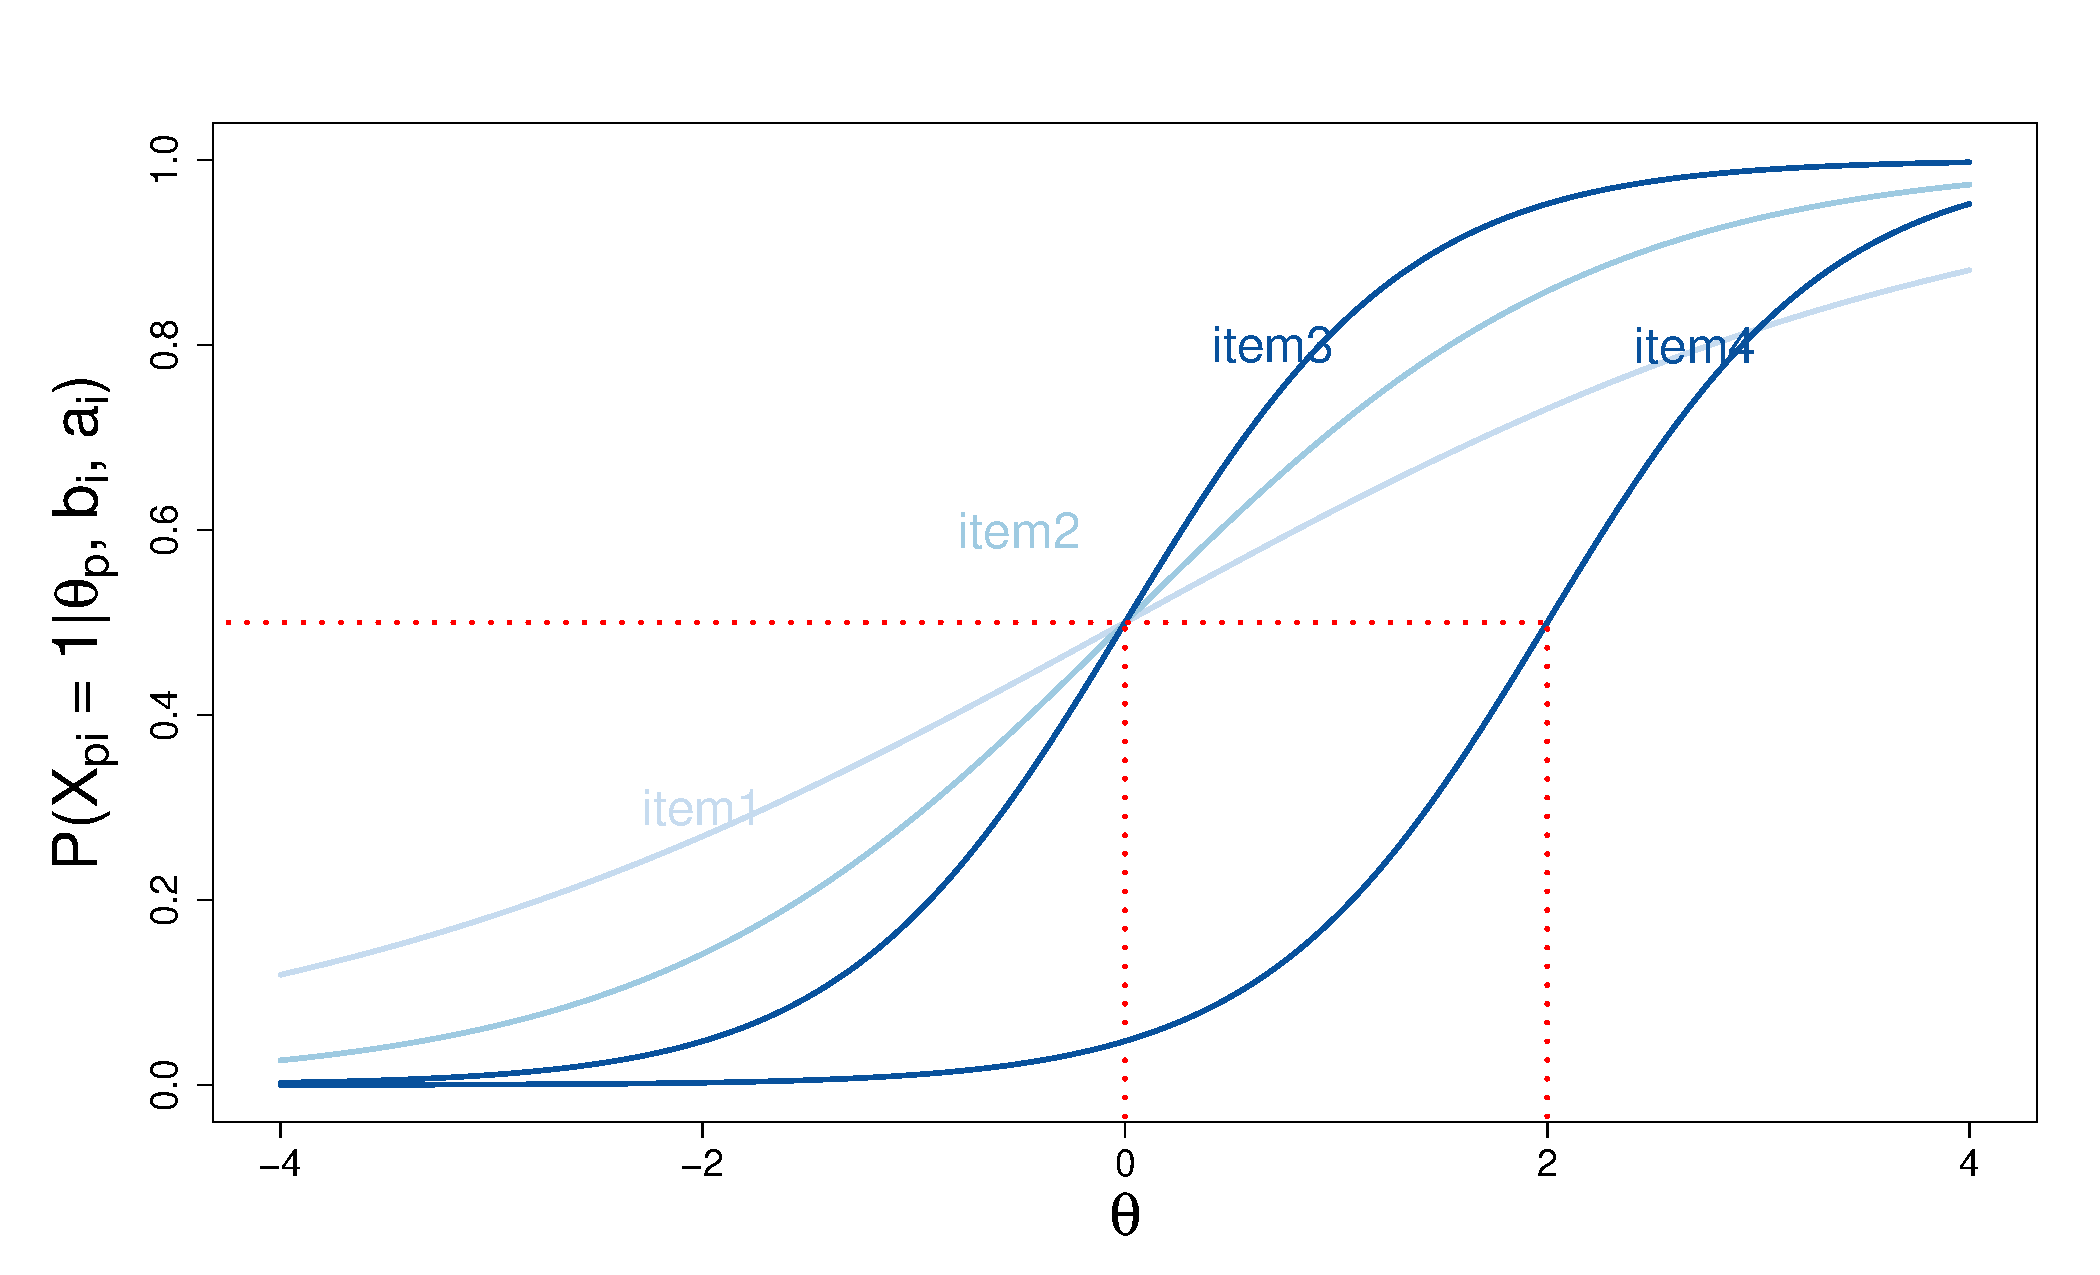
\includegraphics[width=.70\linewidth]{img/ICC-2pl.pdf}
	
	
\end{frame}

\subsection{Item and Test Information Functions}
\begin{frame}
	
	\begin{columns}[T]
	\begin{column}{.5\linewidth}
		\centering
		Item Information Function (IIF): \\	$I_i(\theta) = a_i^2P_i(\theta, b_i, a_i)[1-P_i(\theta, b_i, a_i)]$
		
		\centering
		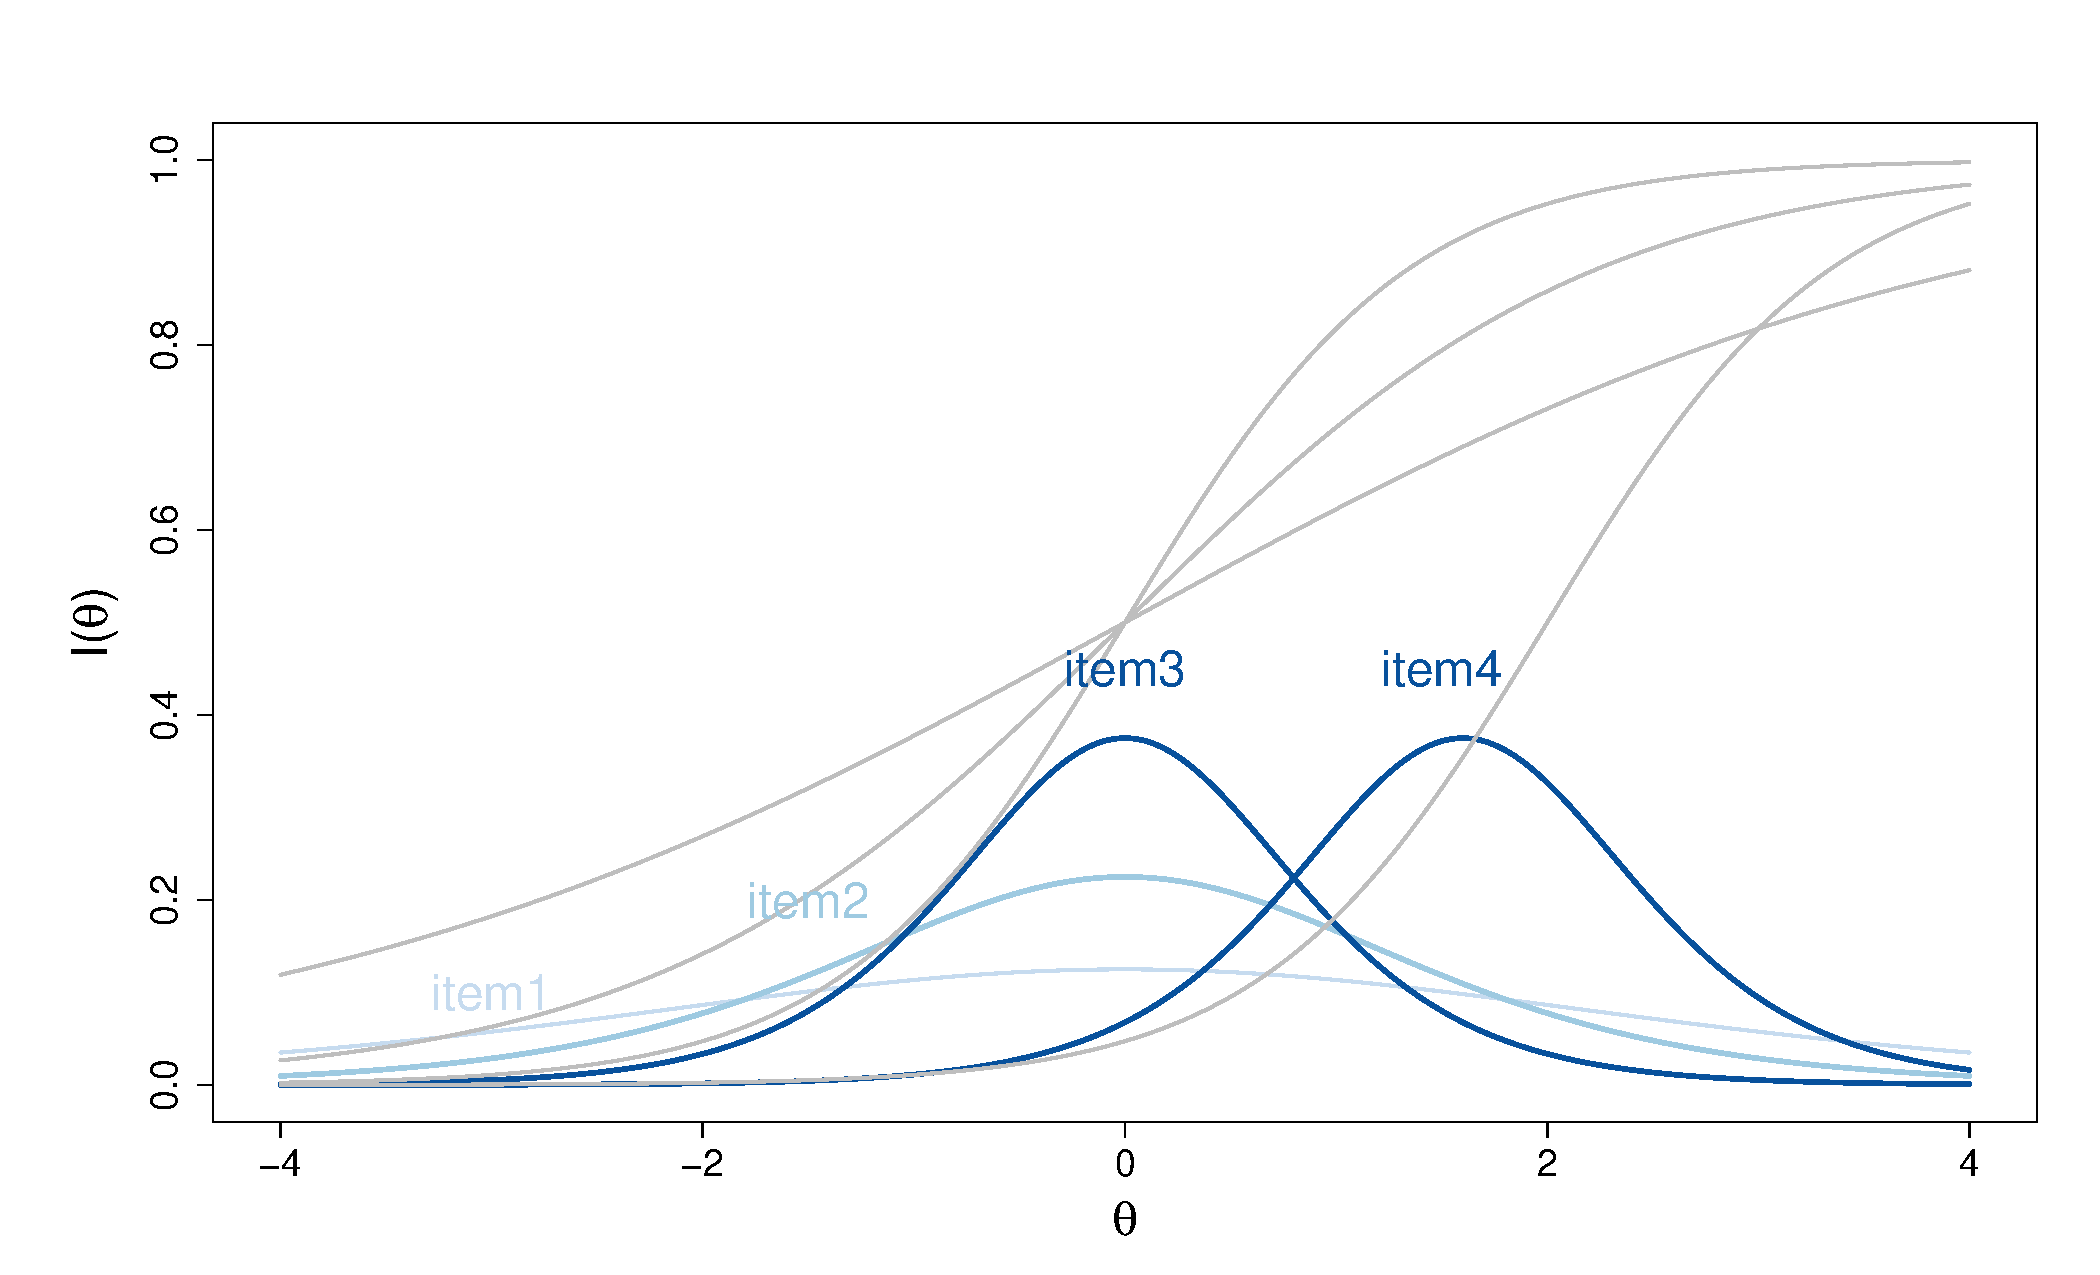
\includegraphics[width=\linewidth]{img/IIF-2pl.pdf}
		
	\end{column}
	\begin{column}{.5\linewidth}
		\centering
		Test Information Function (TIF):	\\	$I(\theta) =  \sum_{i = 1}^{N} I_i(\theta)$
	
	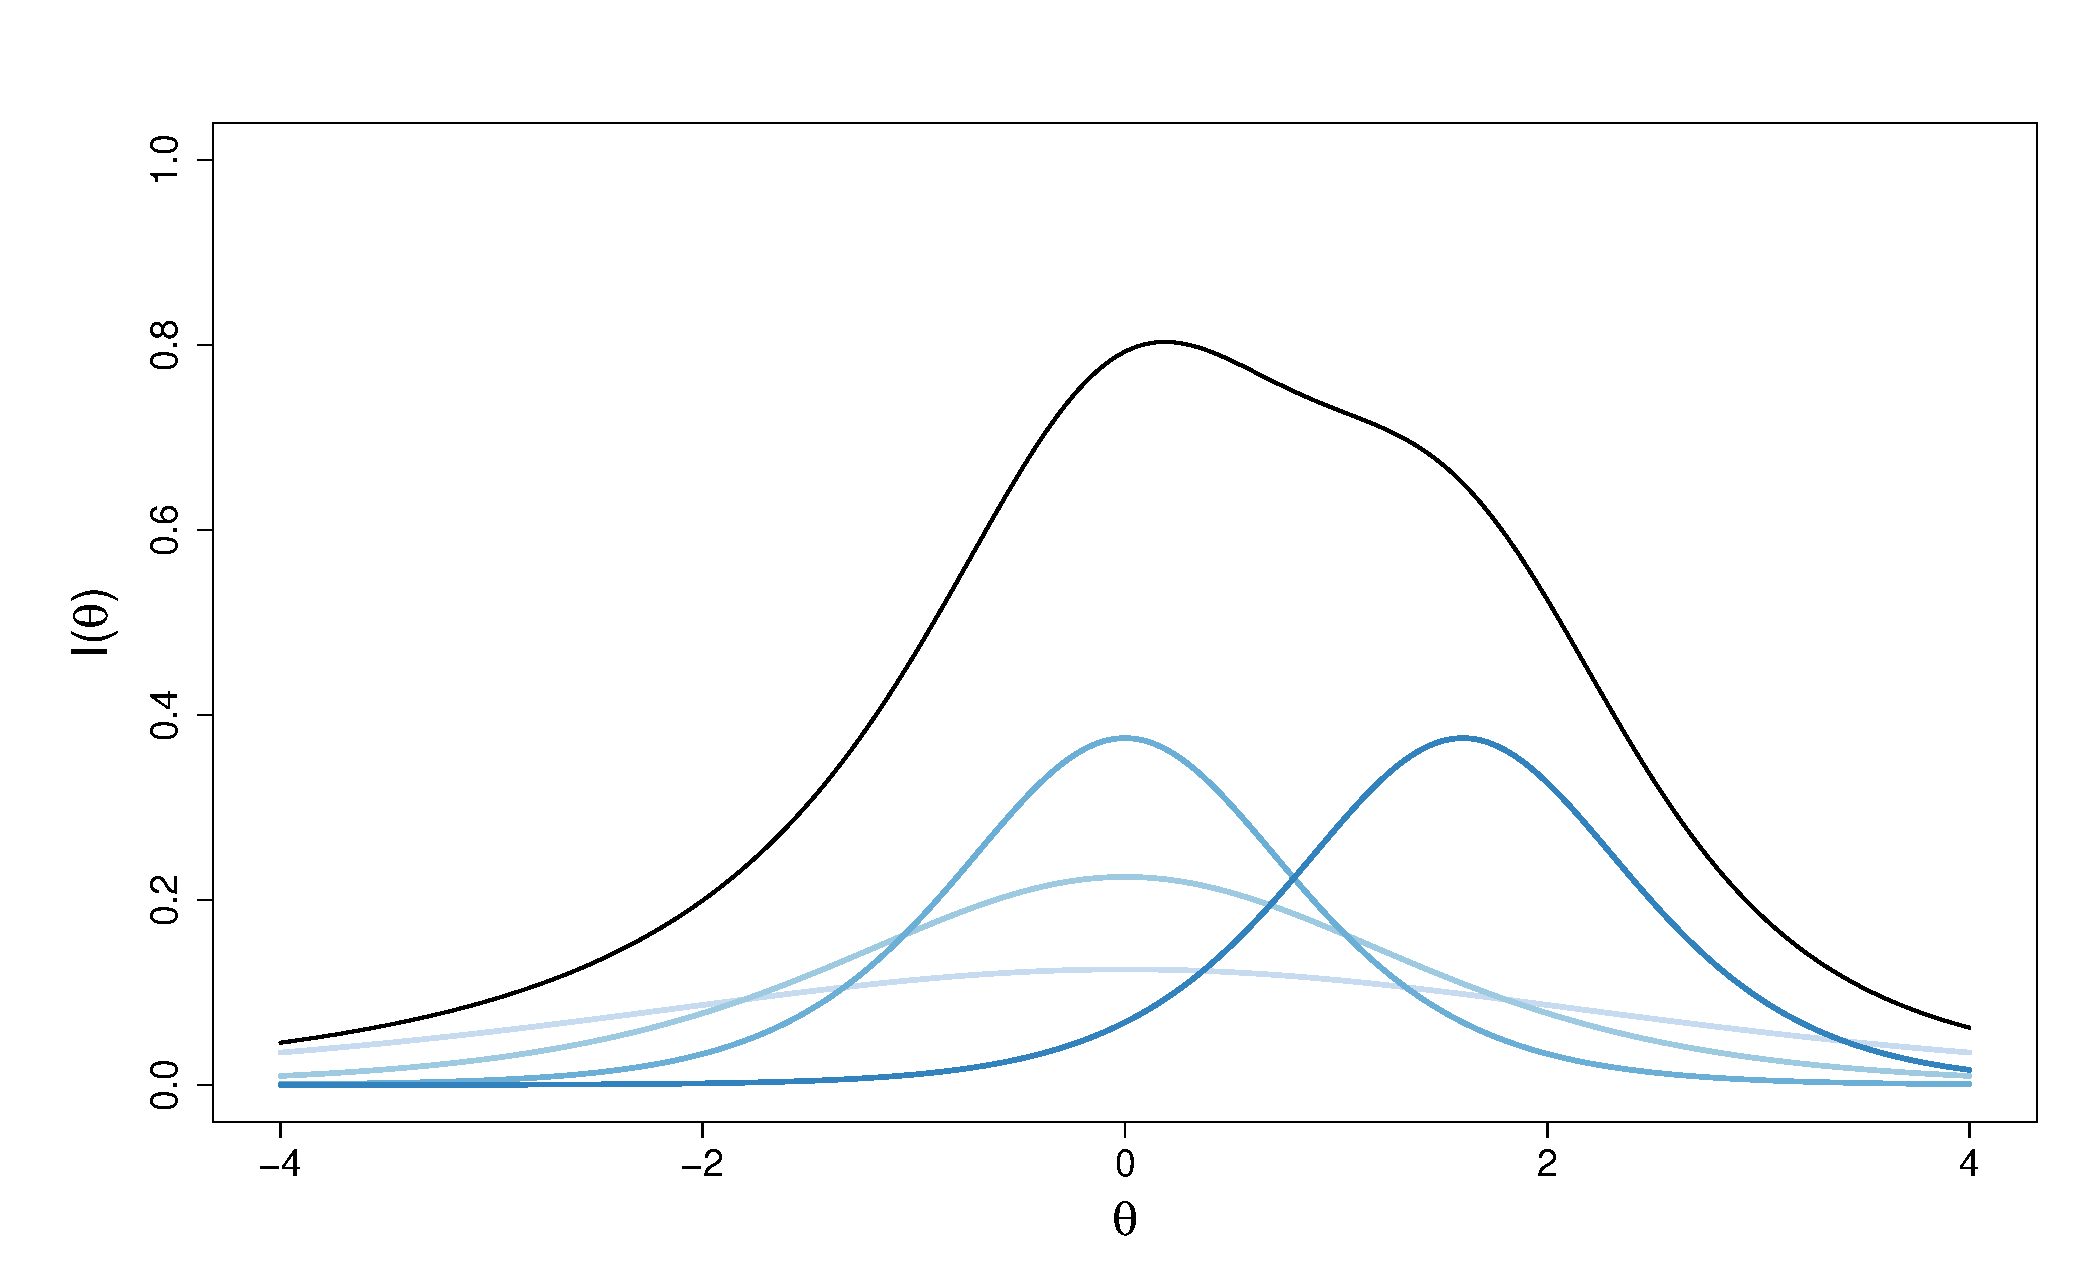
\includegraphics[width=\linewidth]{img/TIF-2pl.pdf}
	
	\end{column}
	\end{columns}
		
\end{frame}

\section{Item Selection Procedures}



\subsection{Item Locating Algorithm -- ILA}
%\begin{frame}
%	
%\textbf{Set up:}
%
%$Q^k$: vector of the item indexes selected for inclusion in the STF up to iteration $k$ ($Q^0 = \emptyset$)
%	
%$\mathbf{TIF}^*$: TIF target 
%
%%$TIF^k = \frac{\sum_{i\in Q^k} IIF_i}{||Q^k||}$, where $||Q^k||$ denotes the cardinality of $Q^k$, 
%$\mathbf{TIF}^0 = (0, 0, \ldots, 0)$ 
%
%
%
%For $k \geq 1$ $\rightarrow$ Iterate and stop if $|\mathbf{TIF}^* - \mathbf{TIF}^k| \geq |\mathbf{TIF}^* - \mathbf{TIF}^{k-1}|$ 
% 
%	\begin{enumerate}
%		%\item  $\Delta_{TIF}^k = |TIF^* - TIF^k|$ %Since at the beginning no items are selected for inclusion in the STF, $Q = \emptyset$ and $||Q|| =0$, so $\Delta_{TIF} = |TIF^* - 0|$. 
%		
%		\item  %A $\theta_{target}$ is determined as the $\theta$ level for which the absolute distance between the $\mathit{TIF}^*$ and $\mathit{TIF}_{TE}$ is maximum, 
%		$\theta_{target} =\argmax{|\mathbf{TIF}^* - \mathbf{TIF}^{k-1}|}$ %At the first iteration, it will be the $\theta$ level with the highest information function. 
%		
%		\item  %The index of the first item to be included in $Q$ is the index of the item whose location is closest to the $\theta_{target}$, 
%	$Q^{k} = Q^{k-1} \cup \argmin_{i \in \{1, \ldots, N\}\setminus Q^{k-1}} |\theta_{target} -b_i|$ \normalcolor
%		
%		\item  $\mathbf{TIF}^{k} = \frac{\sum_{i\in Q^k} \mathbf{IIF}_i}{||Q^k||}$
%		
%		\item $k =  k +1$ 
%		
%	\end{enumerate}
%\end{frame}



%\begin{frame}
%	
%	\textbf{Set up:}
%	
%	$N$: number of items included in the item bank 
%	
%	$Q^k$: Set of item indexes selected for inclusion in the STF up to iteration $k$ ($Q^0 = \emptyset$)
%	
%	$\mathbf{TIF}^*$: TIF target 
%	
%	%$TIF^k = \frac{\sum_{i\in Q^k} IIF_i}{||Q^k||}$, where $||Q^k||$ denotes the cardinality of $Q^k$, 
%	$\mathbf{TIF}^0 = (0, 0, \ldots, 0)$ 
%	
%	
%	
%	For $k \geq 1$:
%	
%	\begin{enumerate}
%		%\item  $\Delta_{TIF}^k = |TIF^* - TIF^k|$ %Since at the beginning no items are selected for inclusion in the STF, $Q = \emptyset$ and $||Q|| =0$, so $\Delta_{TIF} = |TIF^* - 0|$. 
%		
%		\item  %A $\theta_{target}$ is determined as the $\theta$ level for which the absolute distance between the $\mathit{TIF}^*$ and $\mathit{TIF}_{TE}$ is maximum, 
%		$\theta_{target} =\argmax{|\mathbf{TIF}^* - \mathbf{TIF}^{k-1}|}$ %At the first iteration, it will be the $\theta$ level with the highest information function. 
%		
%		\item  %The index of the first item to be included in $Q$ is the index of the item whose location is closest to the $\theta_{target}$, 
%		$Q^{k} = Q^{k-1} \cup \argmin_{i \in \{1, \ldots, N\}\setminus Q^{k-1}} |\theta_{target} -b_i|$ \normalcolor
%		
%		\item  $\mathbf{TIF}^{k} = \frac{\sum_{i\in Q^k} \mathbf{IIF}_i}{||Q^k||}$
%	
%	
%		
%	\end{enumerate}
%	
%	The procedure iterates 1 to 3 until $|\mathbf{TIF}^* - \mathbf{TIF}^k| \geq |\mathbf{TIF}^* - \mathbf{TIF}^{k-1}|$  $\rightarrow$ Stops and returns $Q_{ILA} = Q^{k-1}$
%\end{frame}

\begin{frame}
	
	\begin{columns}[T]
		\begin{column}{.45\linewidth}
			
			\begin{center}
				\textbf{Set up:}
			\end{center}
			
		
			
			\vspace{1.5mm}
			\small
				$N$: number of items included in the item bank 
			
				\vspace{1.5mm}
			$Q^k$: Set of item indexes selected for inclusion in the STF up to iteration $k$ ($Q^0 = \emptyset$)
			
				\vspace{1.5mm}
			$\mathbf{TIF}^*$: TIF target 
			
				\vspace{1.5mm}
			%$TIF^k = \frac{\sum_{i\in Q^k} IIF_i}{||Q^k||}$, where $||Q^k||$ denotes the cardinality of $Q^k$, 
			$\mathbf{TIF}^0 = (0, 0, \ldots, 0)$ 
			
		\end{column}
		
		\begin{column}{.55\linewidth}
			\small 
			\centering
			\textbf{ILA Algorithm:} 
			\scalebox{.5}{
			\begin{tikzpicture}[node distance=2cm]
				
				% Nodes
				\node (start) [startstop] {Start, for $k \geq 1$};
				\node (target) [process, below of=start] {$\theta_{target} = \arg\max |\mathbf{TIF}^* - \mathbf{TIF}^{k-1}|$};
				\node (additem) [process, below of=target] {$Q^{k} = Q^{k-1} \cup \arg\min |\theta_{target} - b_i|$};
				\node (update) [process, below of=additem] {$\mathbf{TIF}^{k} = \frac{\sum_{i \in Q^k} \mathbf{IIF}_i}{||Q^k||}$};
				\node (check) [decision, right of=update, xshift=4cm] {$|\mathbf{TIF}^* - \mathbf{TIF}^k| \geq |\mathbf{TIF}^* - \mathbf{TIF}^{k-1}|$?};
				\node (stop) [startstop, below of=check, yshift=-3.5cm] {Stop \& Return $Q_{ILA} = Q^{k-1}$};
				
				% Arrows
				\draw [arrow] (start) -- (target);
				\draw [arrow] (target) -- (additem);
				\draw [arrow] (additem) -- (update);
				\draw [arrow] (update) -- (check);
				\draw [arrow] (check) -- node[anchor=east] {Yes} (stop);
				\draw [arrow] (check.east) -- ++(1,0) -- ++(0,4) -- node[anchor=north] {No} (target.east);
				
			\end{tikzpicture}
		}
		
		\end{column}
	\end{columns}
	


\end{frame}

\subsection{Brute Force Procedure -- BFP}
\begin{frame}

%	$\binom{N}{l}$: number of STFs of length $l = \{1, \ldots N-1\}$ items 
	
%	For each of the $\binom{N}{l}$ combinations of $l$ items ($1 \leq l \leq N-1$), denoted by $m_l$, iterate: 
 
 %Let $Q^{m_l}$ be the set of $l$ items
 
 For each $Q_m \subset Q$ with $Q_m \neq \emptyset$, calculate:
 
 \begin{enumerate}
 	\item $\mathbf{TIF}^{Q_m} =  \dfrac{\sum_{i \in Q_m} IIF_i}{||Q_m||}$
 	\item $\overline{\Delta}_{\mathbf{TIF}^{Q_m}} =  \mathit{mean}(|\mathbf{TIF}^* - \mathbf{TIF}^{Q_m}|)$
 \end{enumerate}
	
	$Q_{BFP} = \argmin_{\emptyset \neq Q_m \subset Q} \overline{\Delta}_{\mathbf{TIF}^{Q_m}}$
	
	%The best STF is the one with the lowest value of $\overline{\Delta}_{TIF}$, that is the one that presents the lowest absolute distance from the TIF target.
\end{frame}

\section{Simulation Study}

\subsection{Simulation design}
\begin{frame}
	
\small
\textbf{100 iterations}:
	
	\begin{enumerate}
		\item  Generate an item bank $B$ of $N = 6$ items: 
		\begin{itemize}
			\item Difficulty parameters: $\mathcal{U}(-3, 3)$
			\item Discrimination parameters:  $\mathcal{U}(.90, 2.0)$
		\end{itemize} 
		
		\item  Random item selections of lengths $l$ from $B$ ($M_l = 3.34 \pm 1.13$) + modification parameters $\mathcal{U}(-0.20, 0.20)$ $\rightarrow$ $\mathbf{TIF}^*$ 
		
		\item  Considering $\mathbf{TIF}^*$ at Step 2 and item parameters at Step 1:
		\begin{itemize}
			\item ILA  $\rightarrow$ \emph{Forwardly searches} %the item selection best able to recover the $TIF^*$
			\item BFP  $\rightarrow$ \emph{Systematically tests} % every item combination to find the one best able to recover $TIF^*$. \\ 
		%	\small $N=6$ $\rightarrow$ $62$ STFs
		\end{itemize}
		
	\end{enumerate}

\textbf{Comparison}:
	
	\begin{itemize}
		\item $||Q_{\text{BFP}}|| - ||Q_{\text{ILA}}||$ 
		\item Percentile rank of the distance $\mathbf{TIF}_{\text{BFP}} - \mathbf{TIF}_{\text{ILA}}$   
	\end{itemize}
	

\end{frame}




\subsection{Results}

\subsection*{$||Q_{BFP}||$ vs. $||Q_{ILA}||$}

\begin{frame}
 $||Q_{\text{BFP}}|| - ||Q_{\text{ILA}}|| = 0$ in 57\% of cases % $\rightarrow$ 72\% same item selection
	\begin{figure}
		\centering
		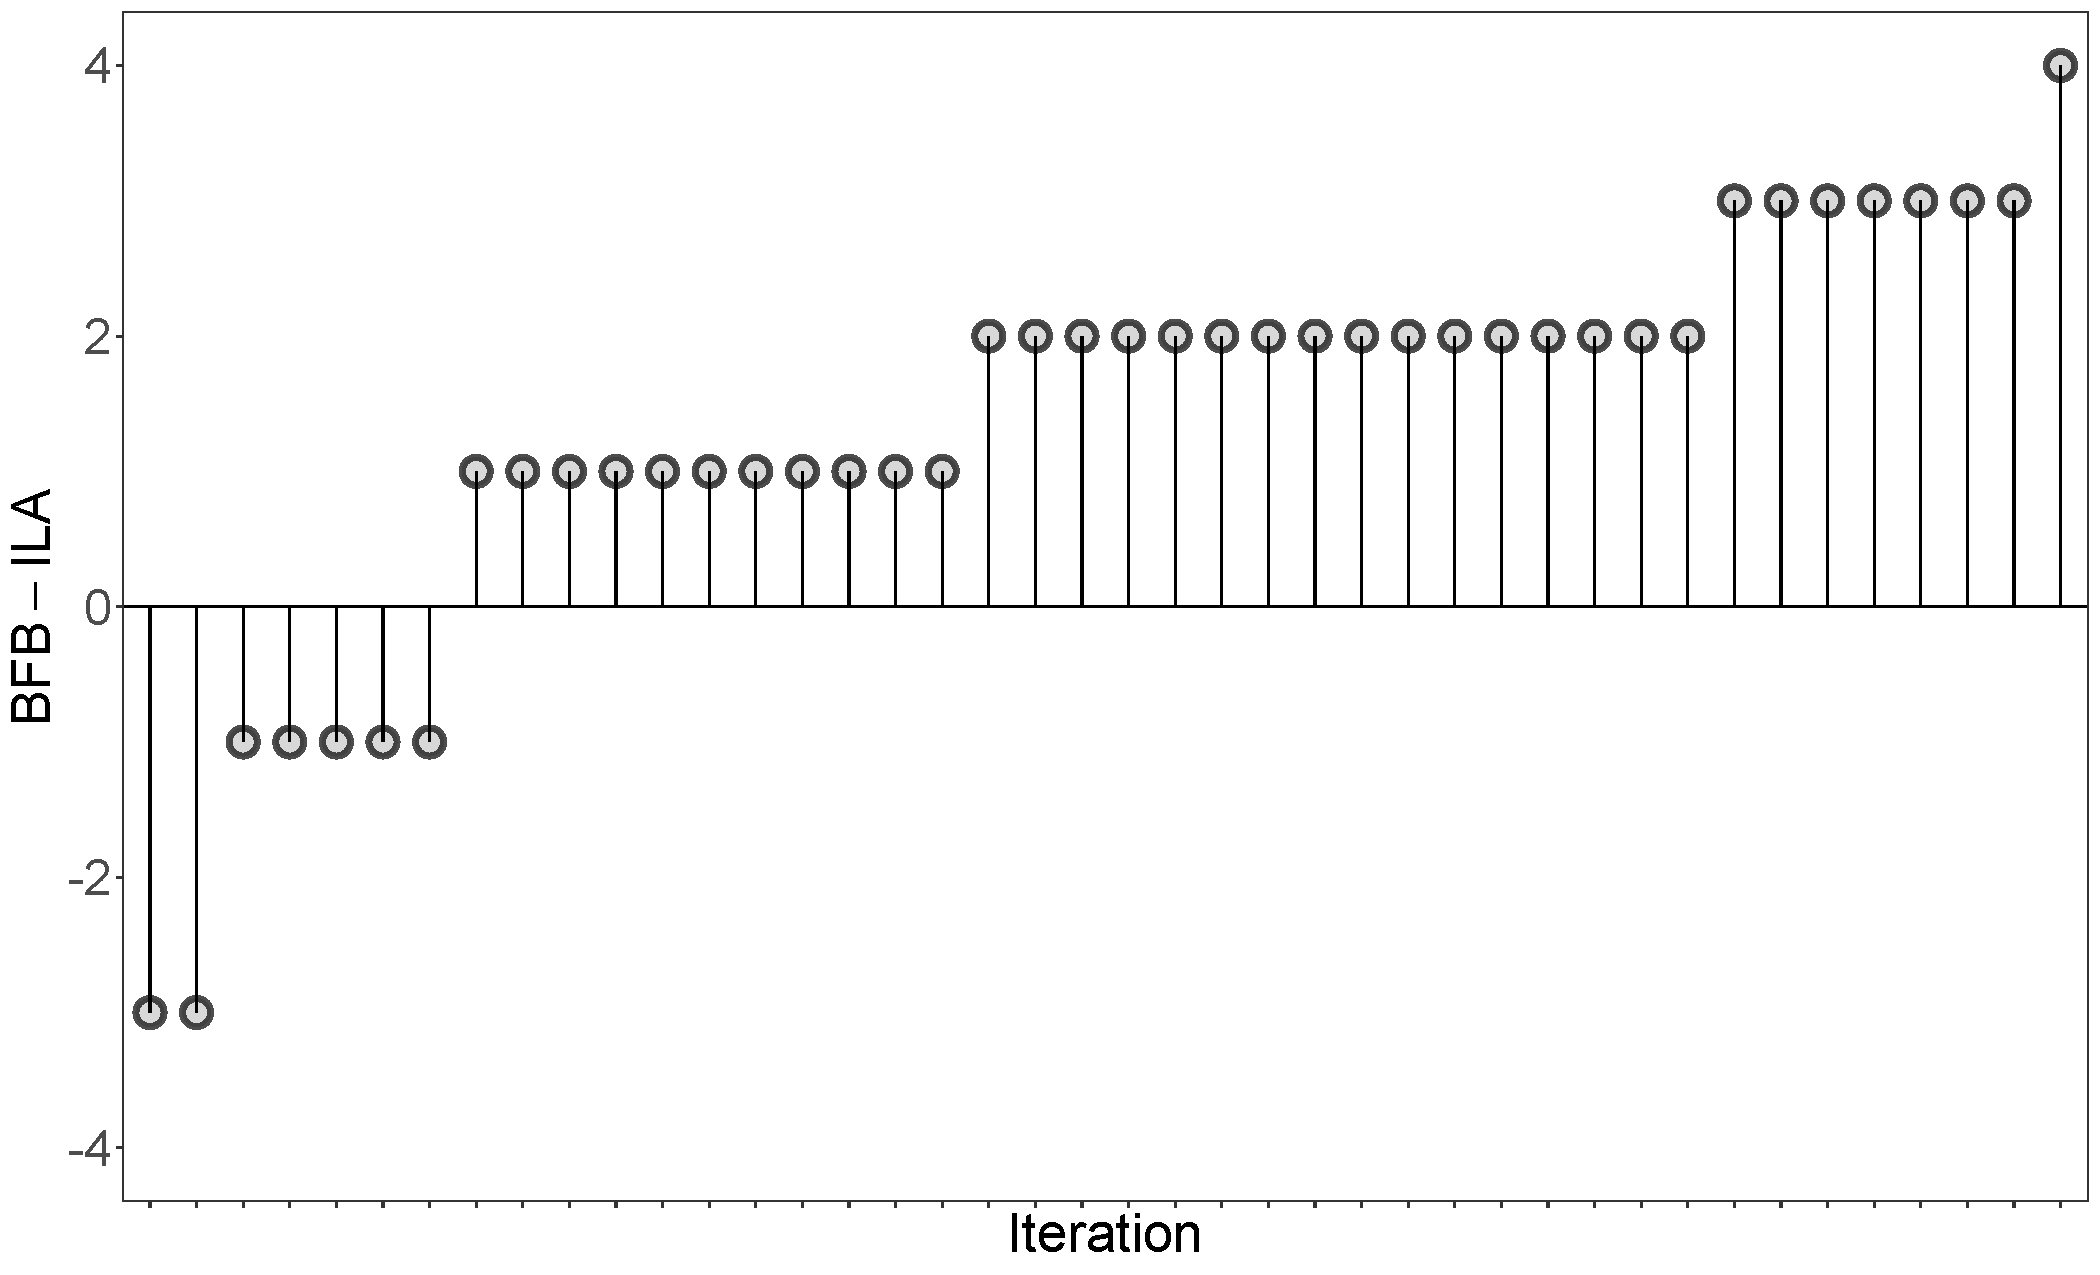
\includegraphics[width=.80\linewidth]{img/bfp-ila}
		%\caption{43\% $\rightarrow$ $||Q_{\text{BFP}}|| - ||Q_{\text{ILA}}|| \neq 0$ }
	\end{figure}
\end{frame}

\subsection*{Distance}

\begin{frame}
	\begin{figure}
		\centering
		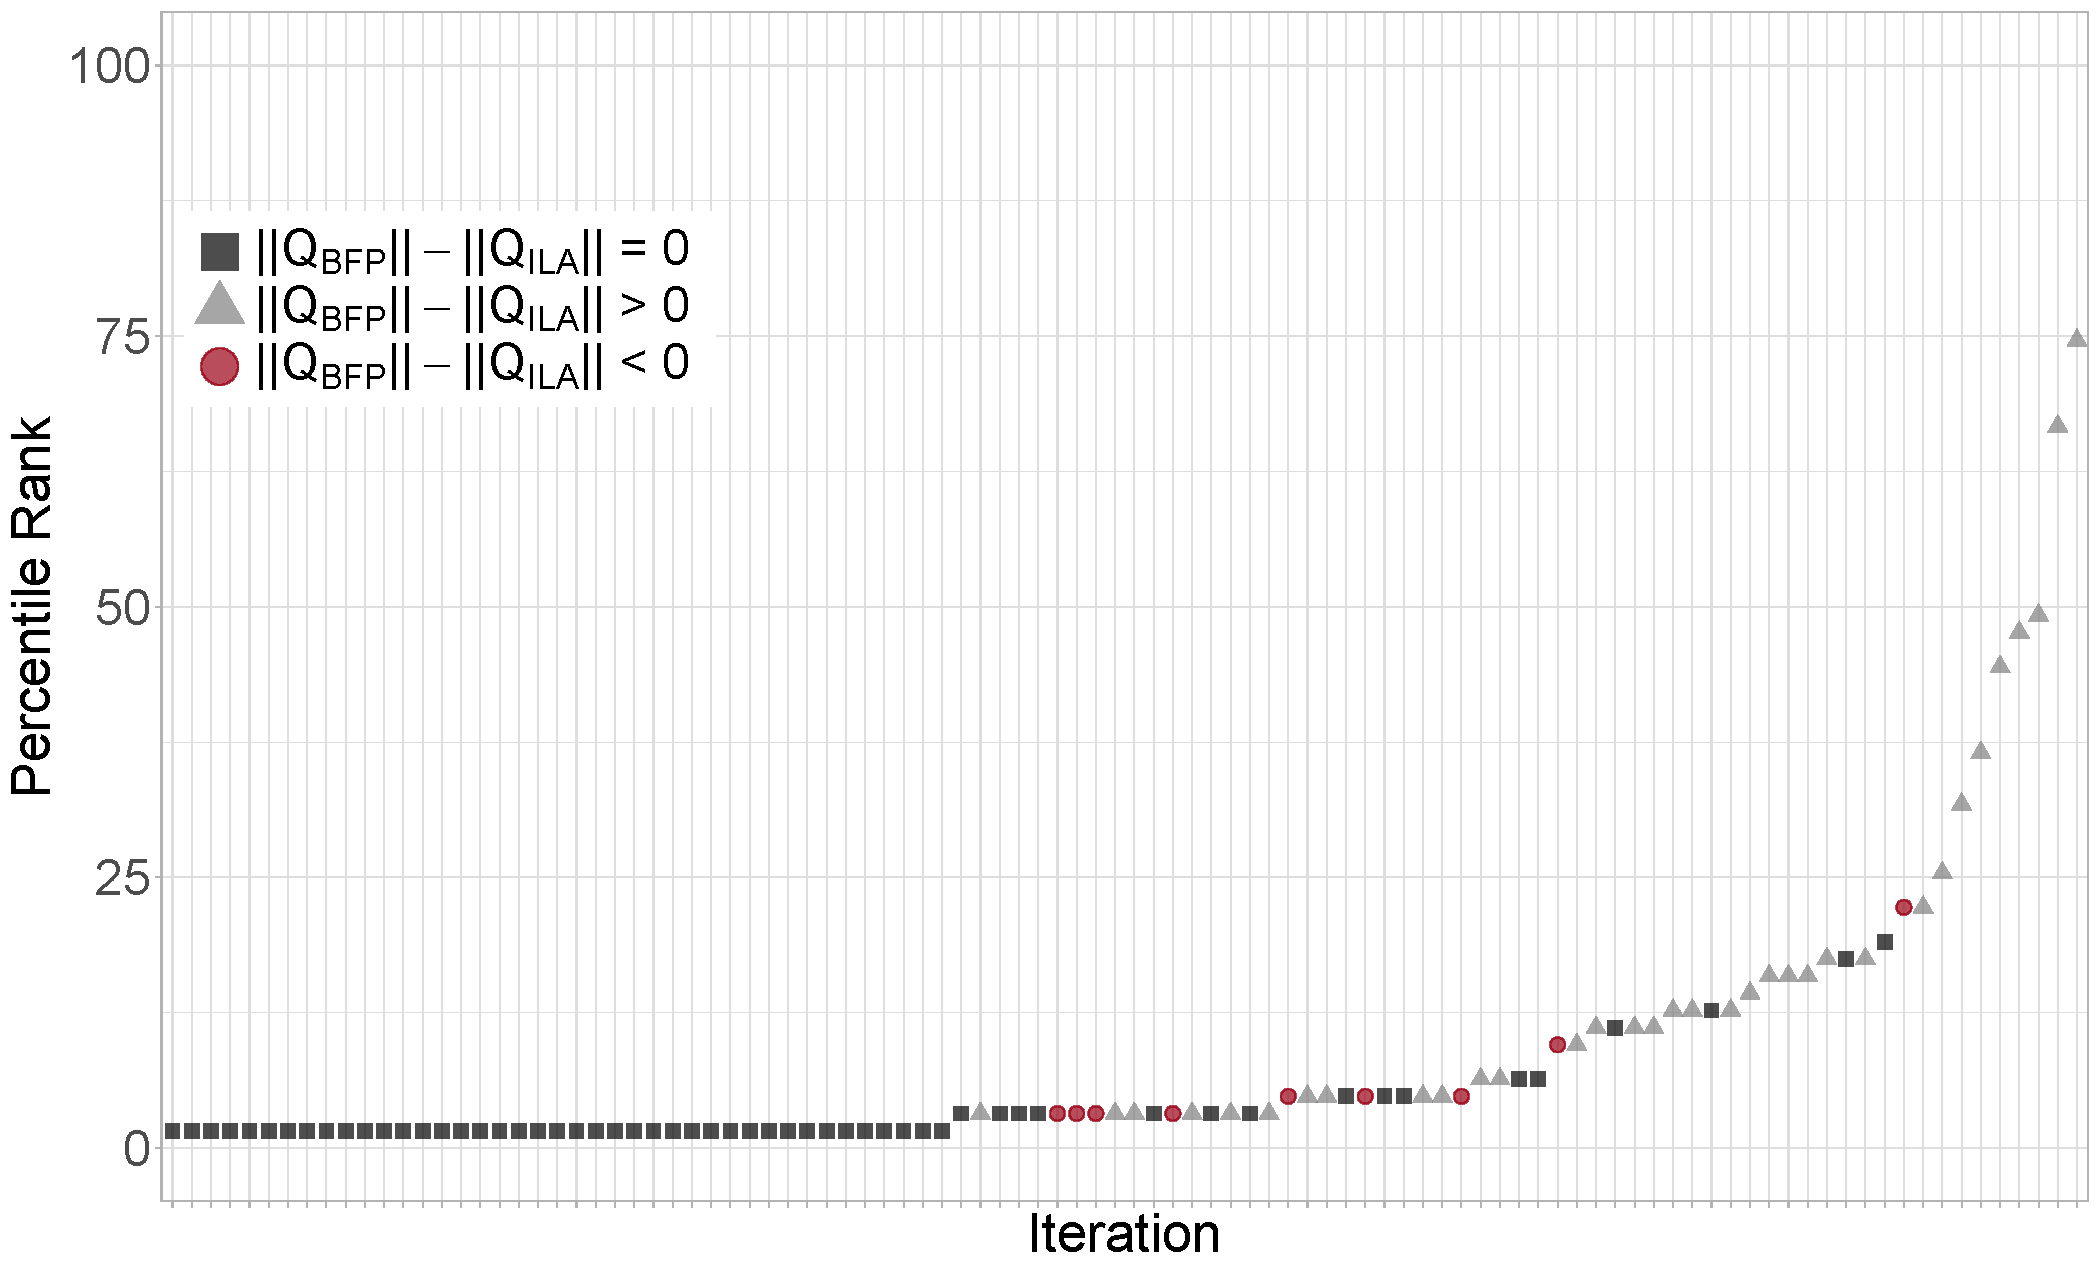
\includegraphics[width=\linewidth]{img/rp}
	\end{figure}
\end{frame}

\subsection*{TIF comparison}

\begin{frame}
	
	\begin{columns}[T]
	\begin{column}{.50\linewidth}

	\centering
		\footnotesize{$||Q_{\text{BFP}}|| = ||Q_{\text{ILA}}||$, $Q_{\text{BFP}} \neq Q_{\text{ILA}}$, $RP = 3.17$}
	
	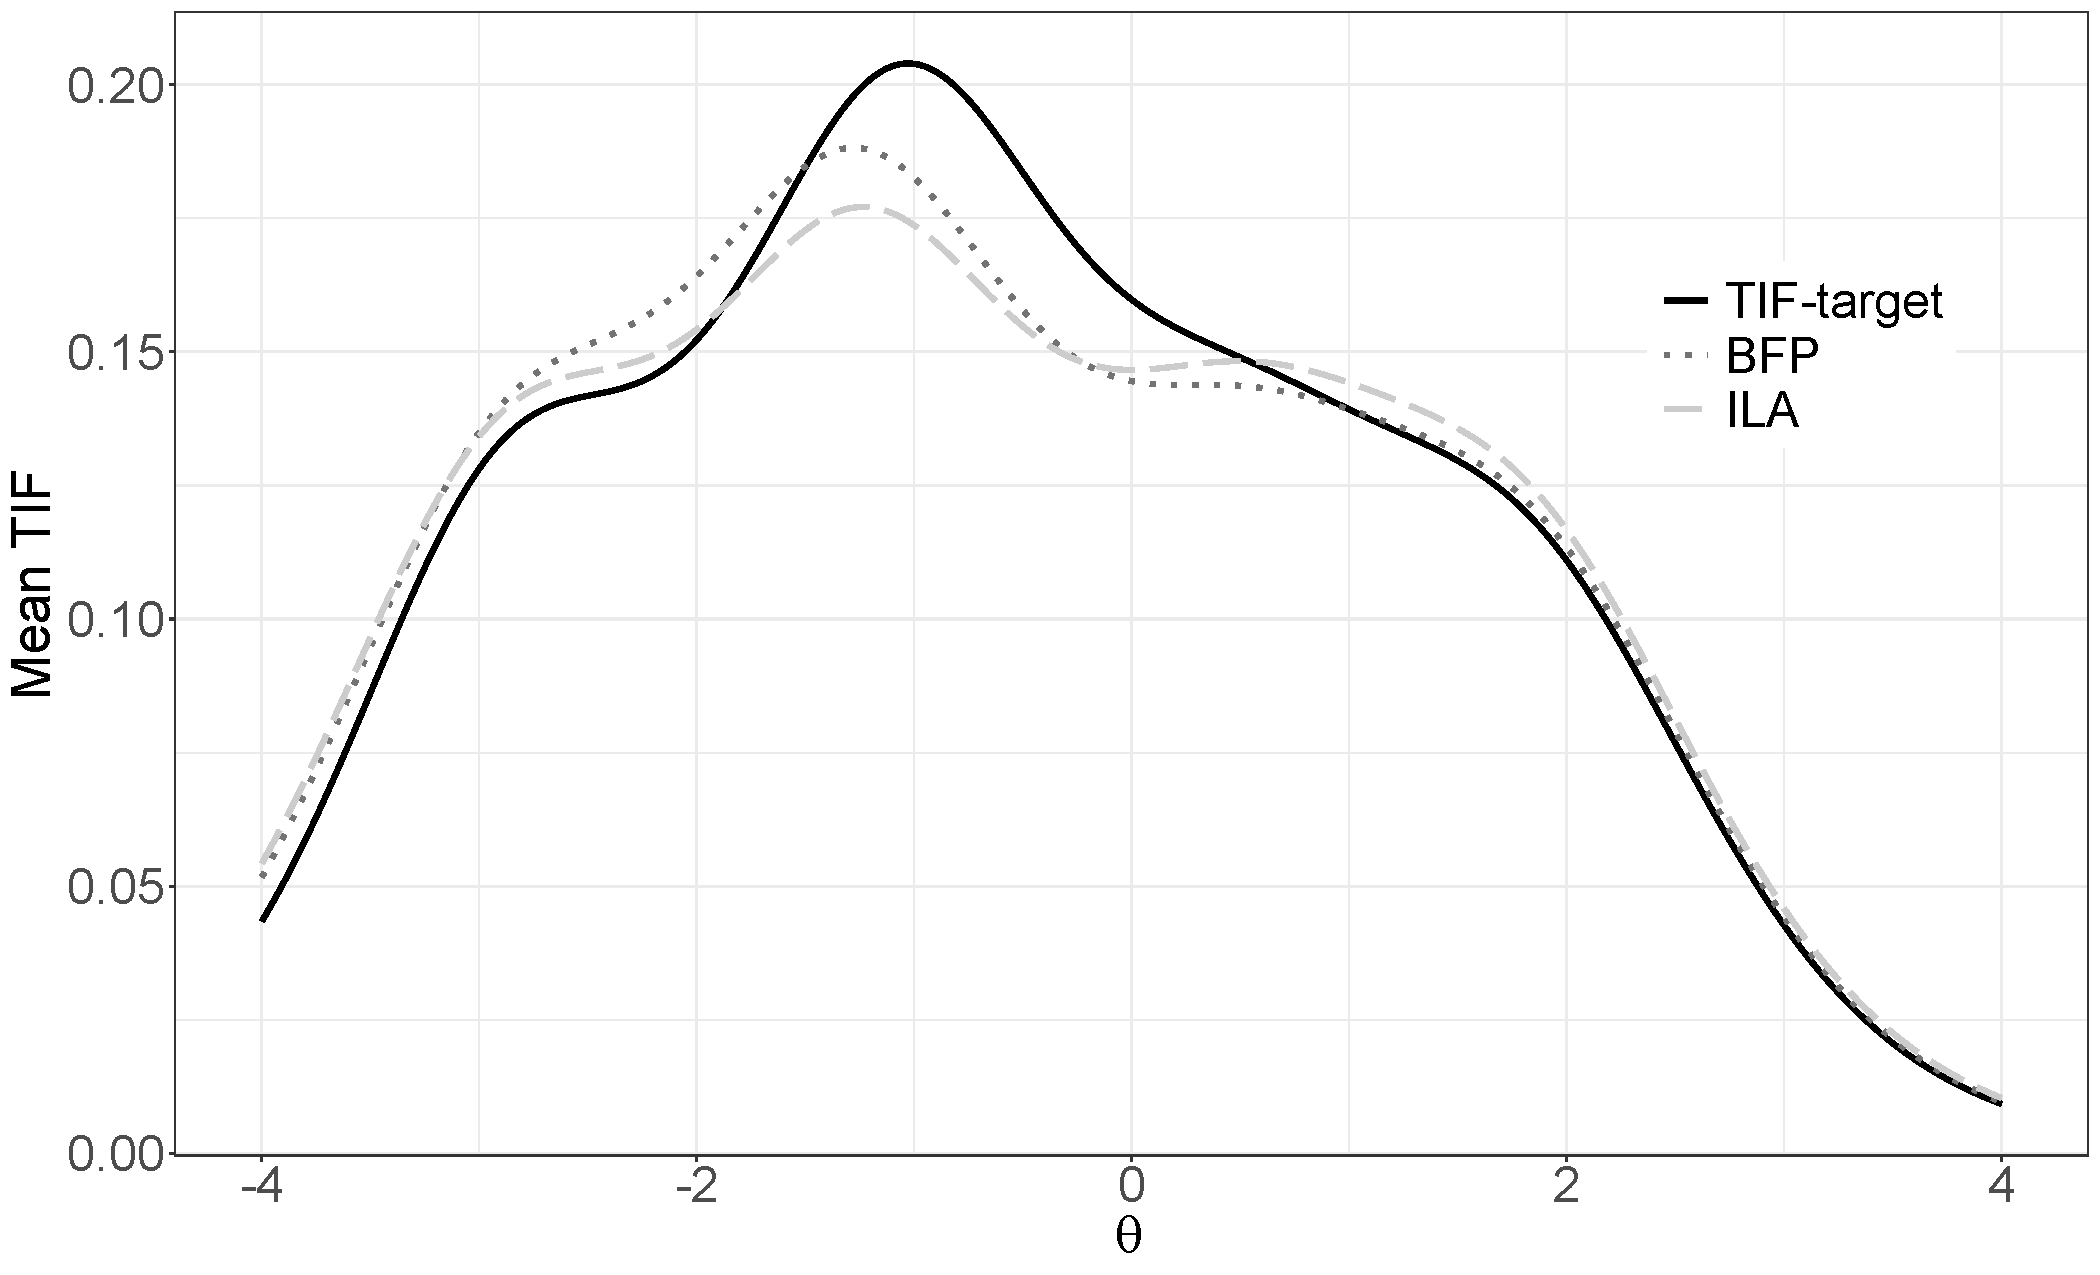
\includegraphics[width=.80\linewidth]{img/equalClose.pdf}	


\centering
\footnotesize{$||Q_{\text{BFP}}|| < ||Q_{\text{ILA}}||$, $RP = 3.17$}
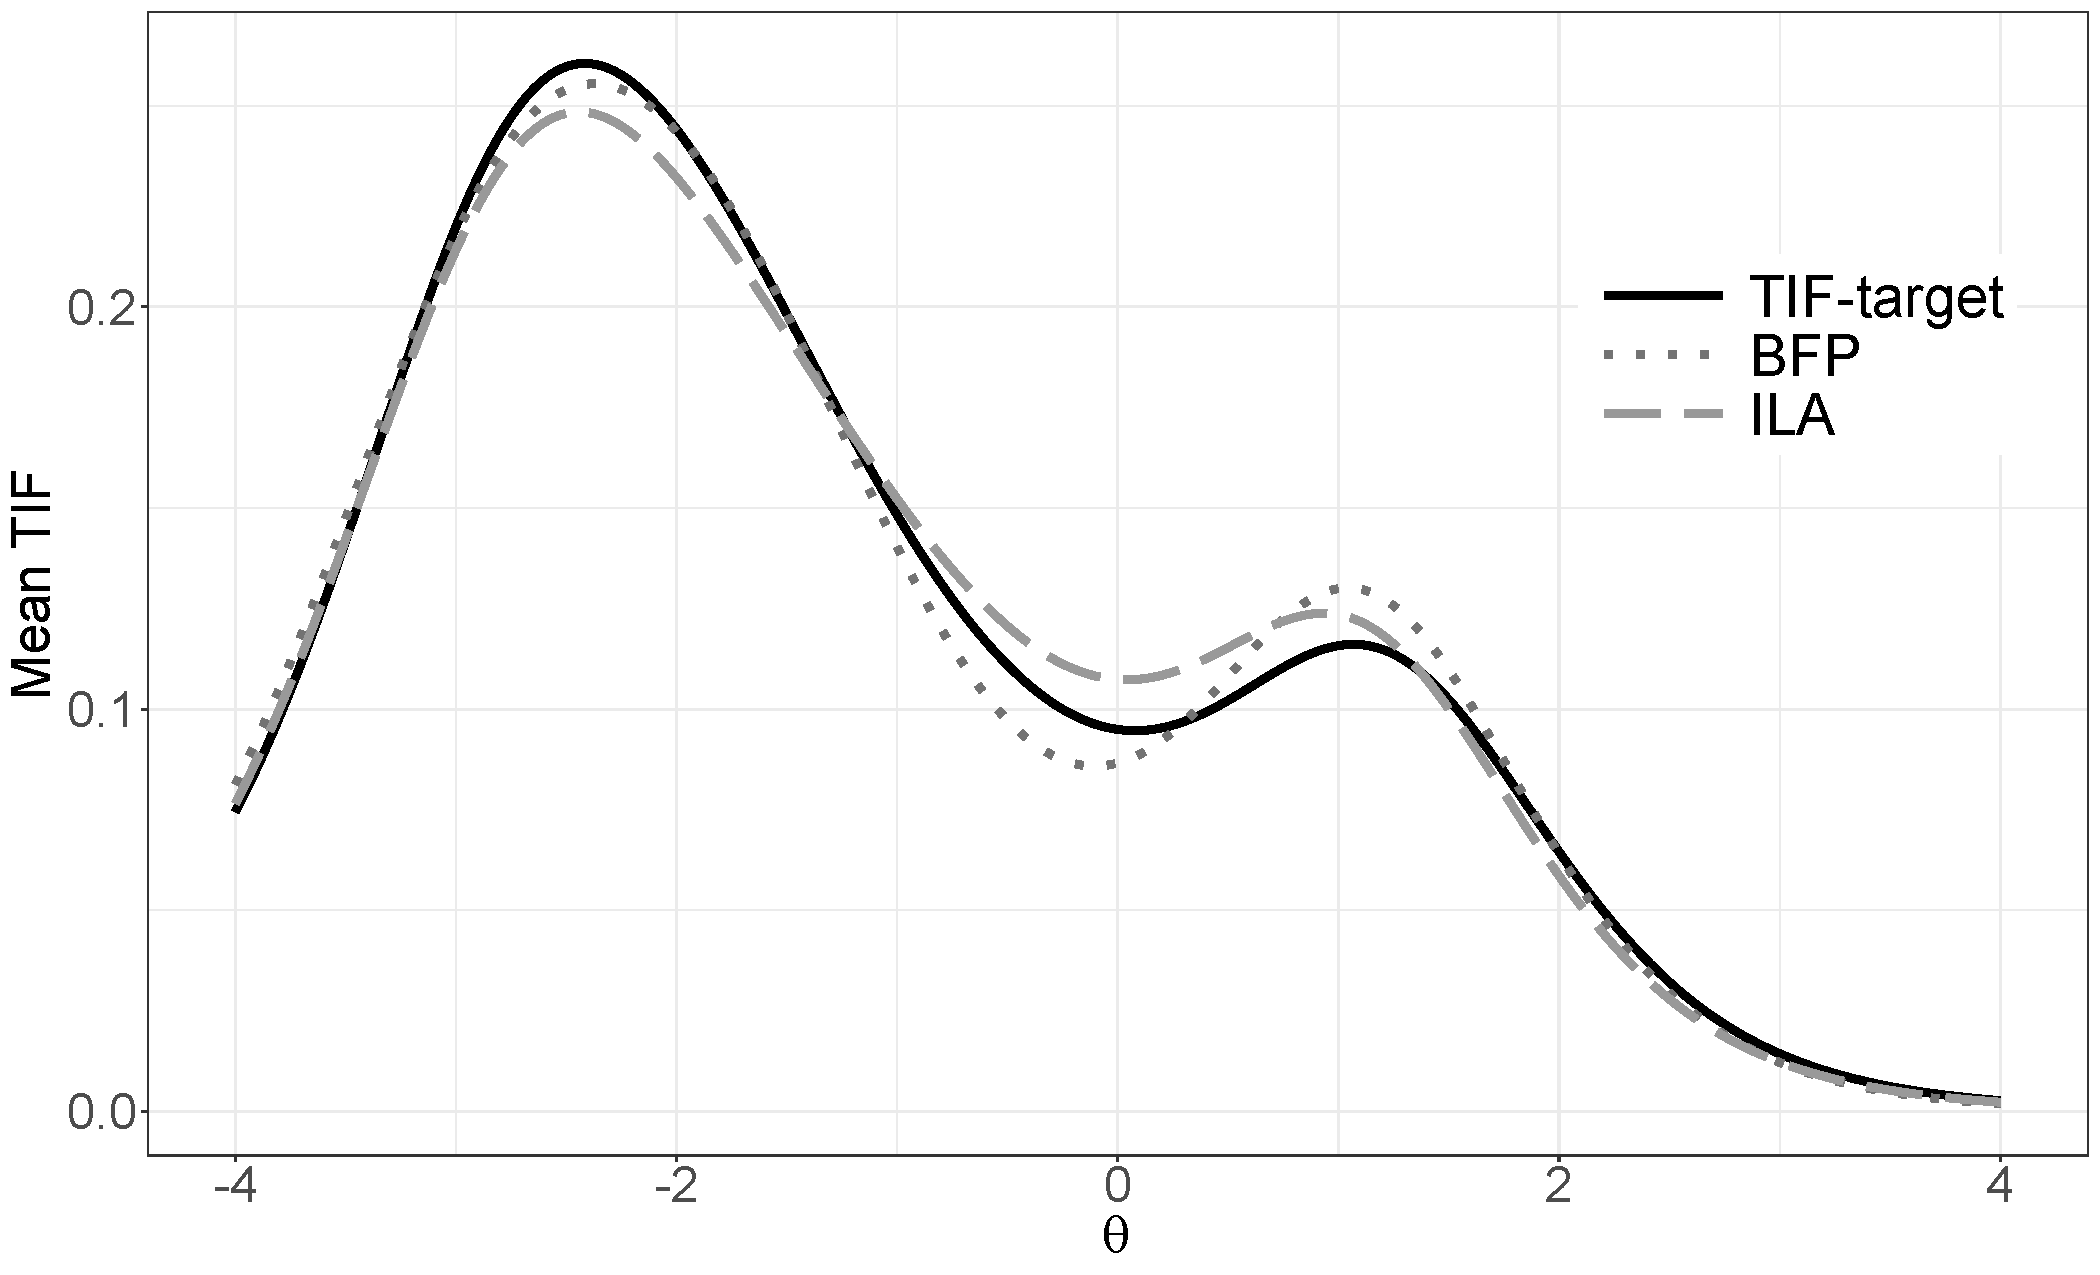
\includegraphics[width=.80\linewidth]{img/moreClose.pdf}	



	\end{column}
	
		\begin{column}{.50\linewidth}
		
		\centering
				\footnotesize{$||Q_{\text{BFP}}|| > ||Q_{\text{ILA}}||$, $RP = 4.76$}
		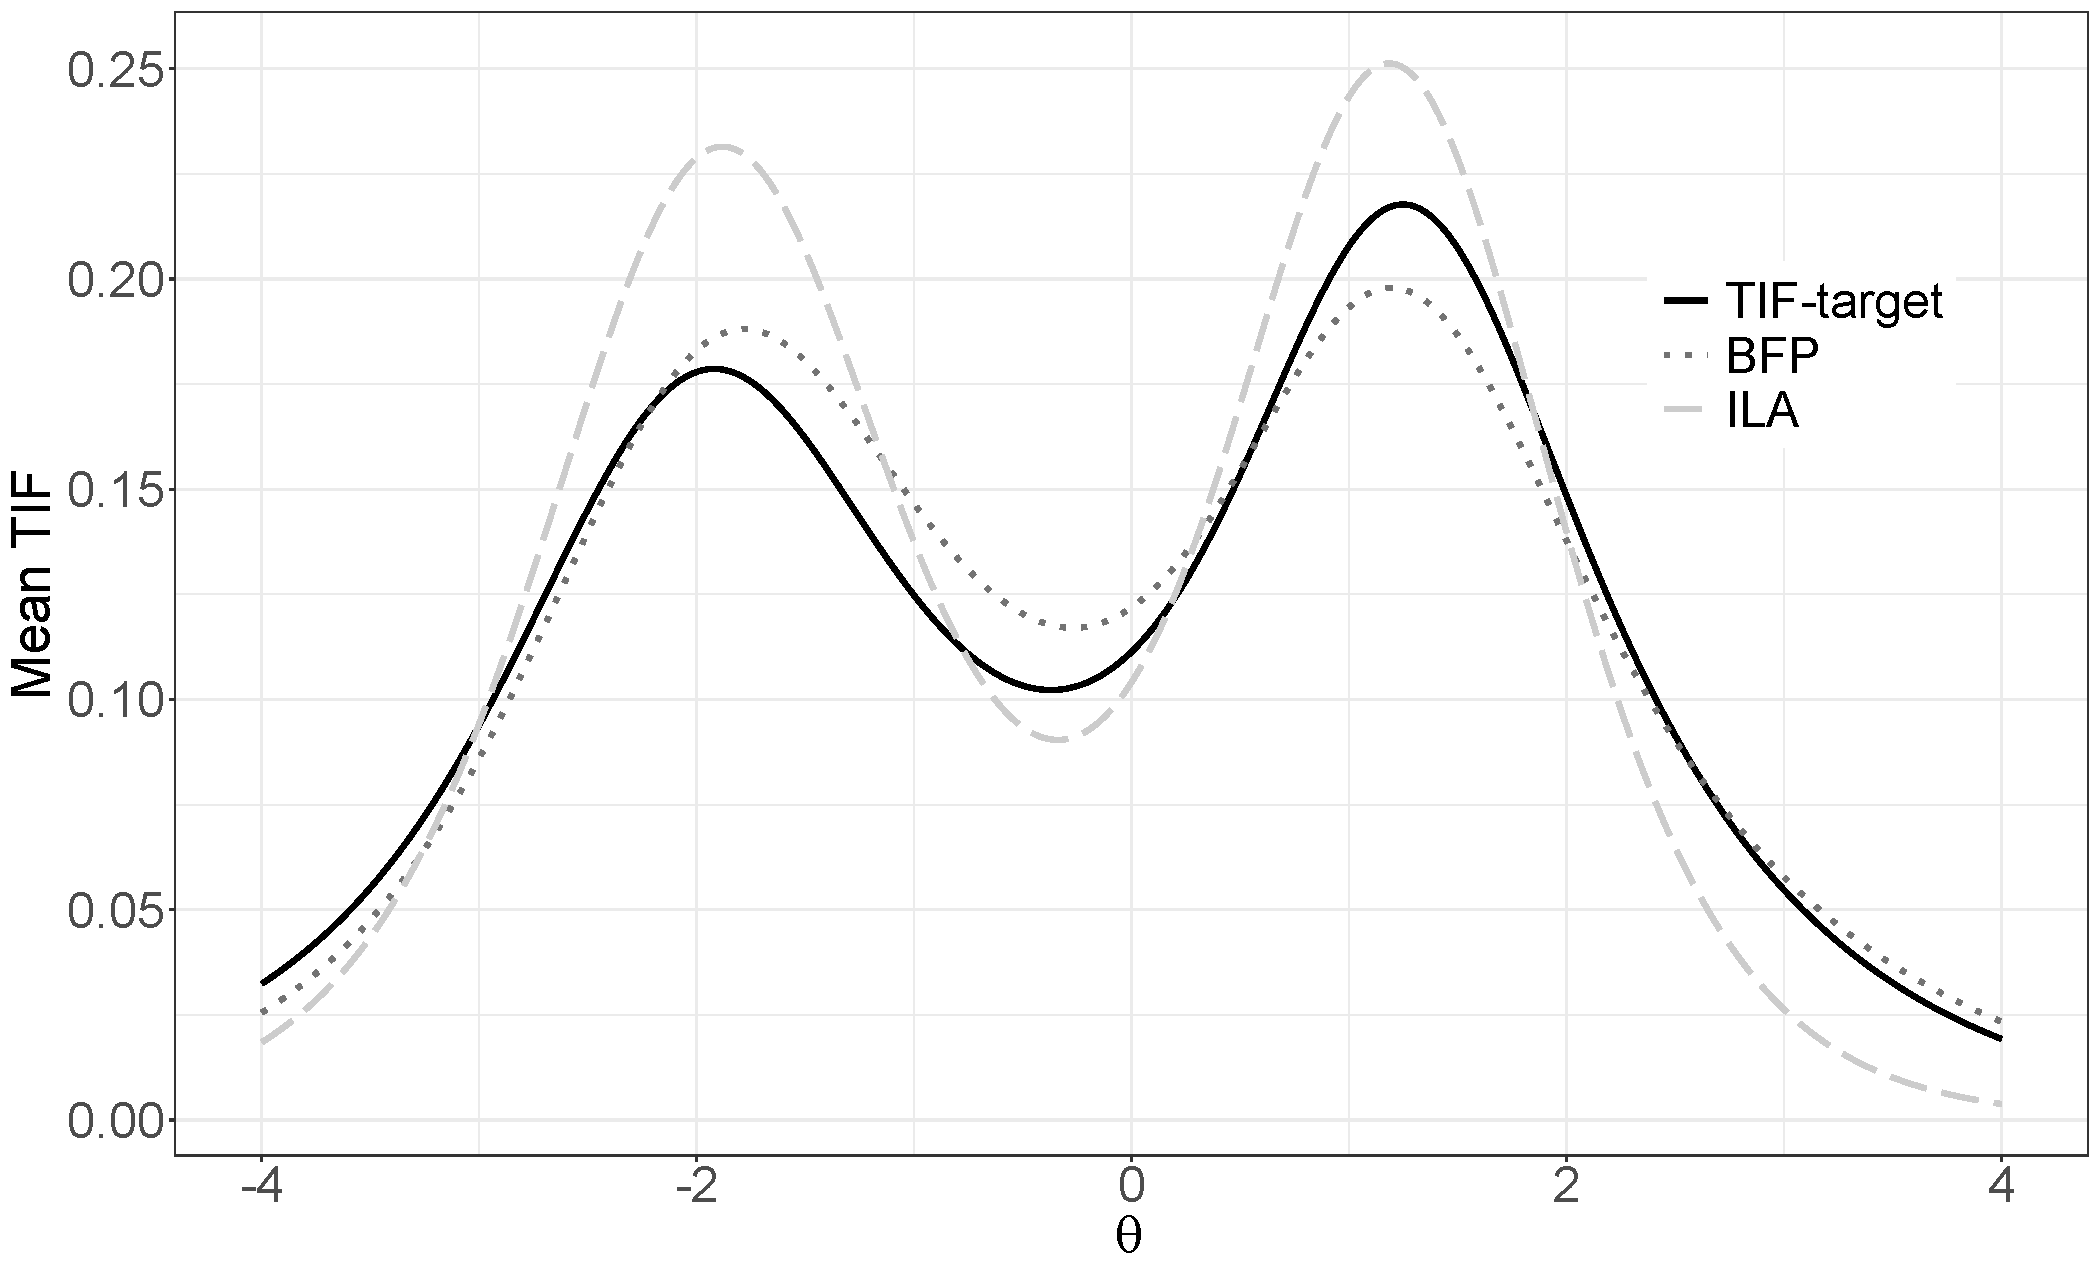
\includegraphics[width=.80\linewidth]{img/lessClose.pdf}	

		
				\centering
						\footnotesize{$||Q_{\text{BFP}}|| > ||Q_{\text{ILA}}||$, $RP=12.70$}
		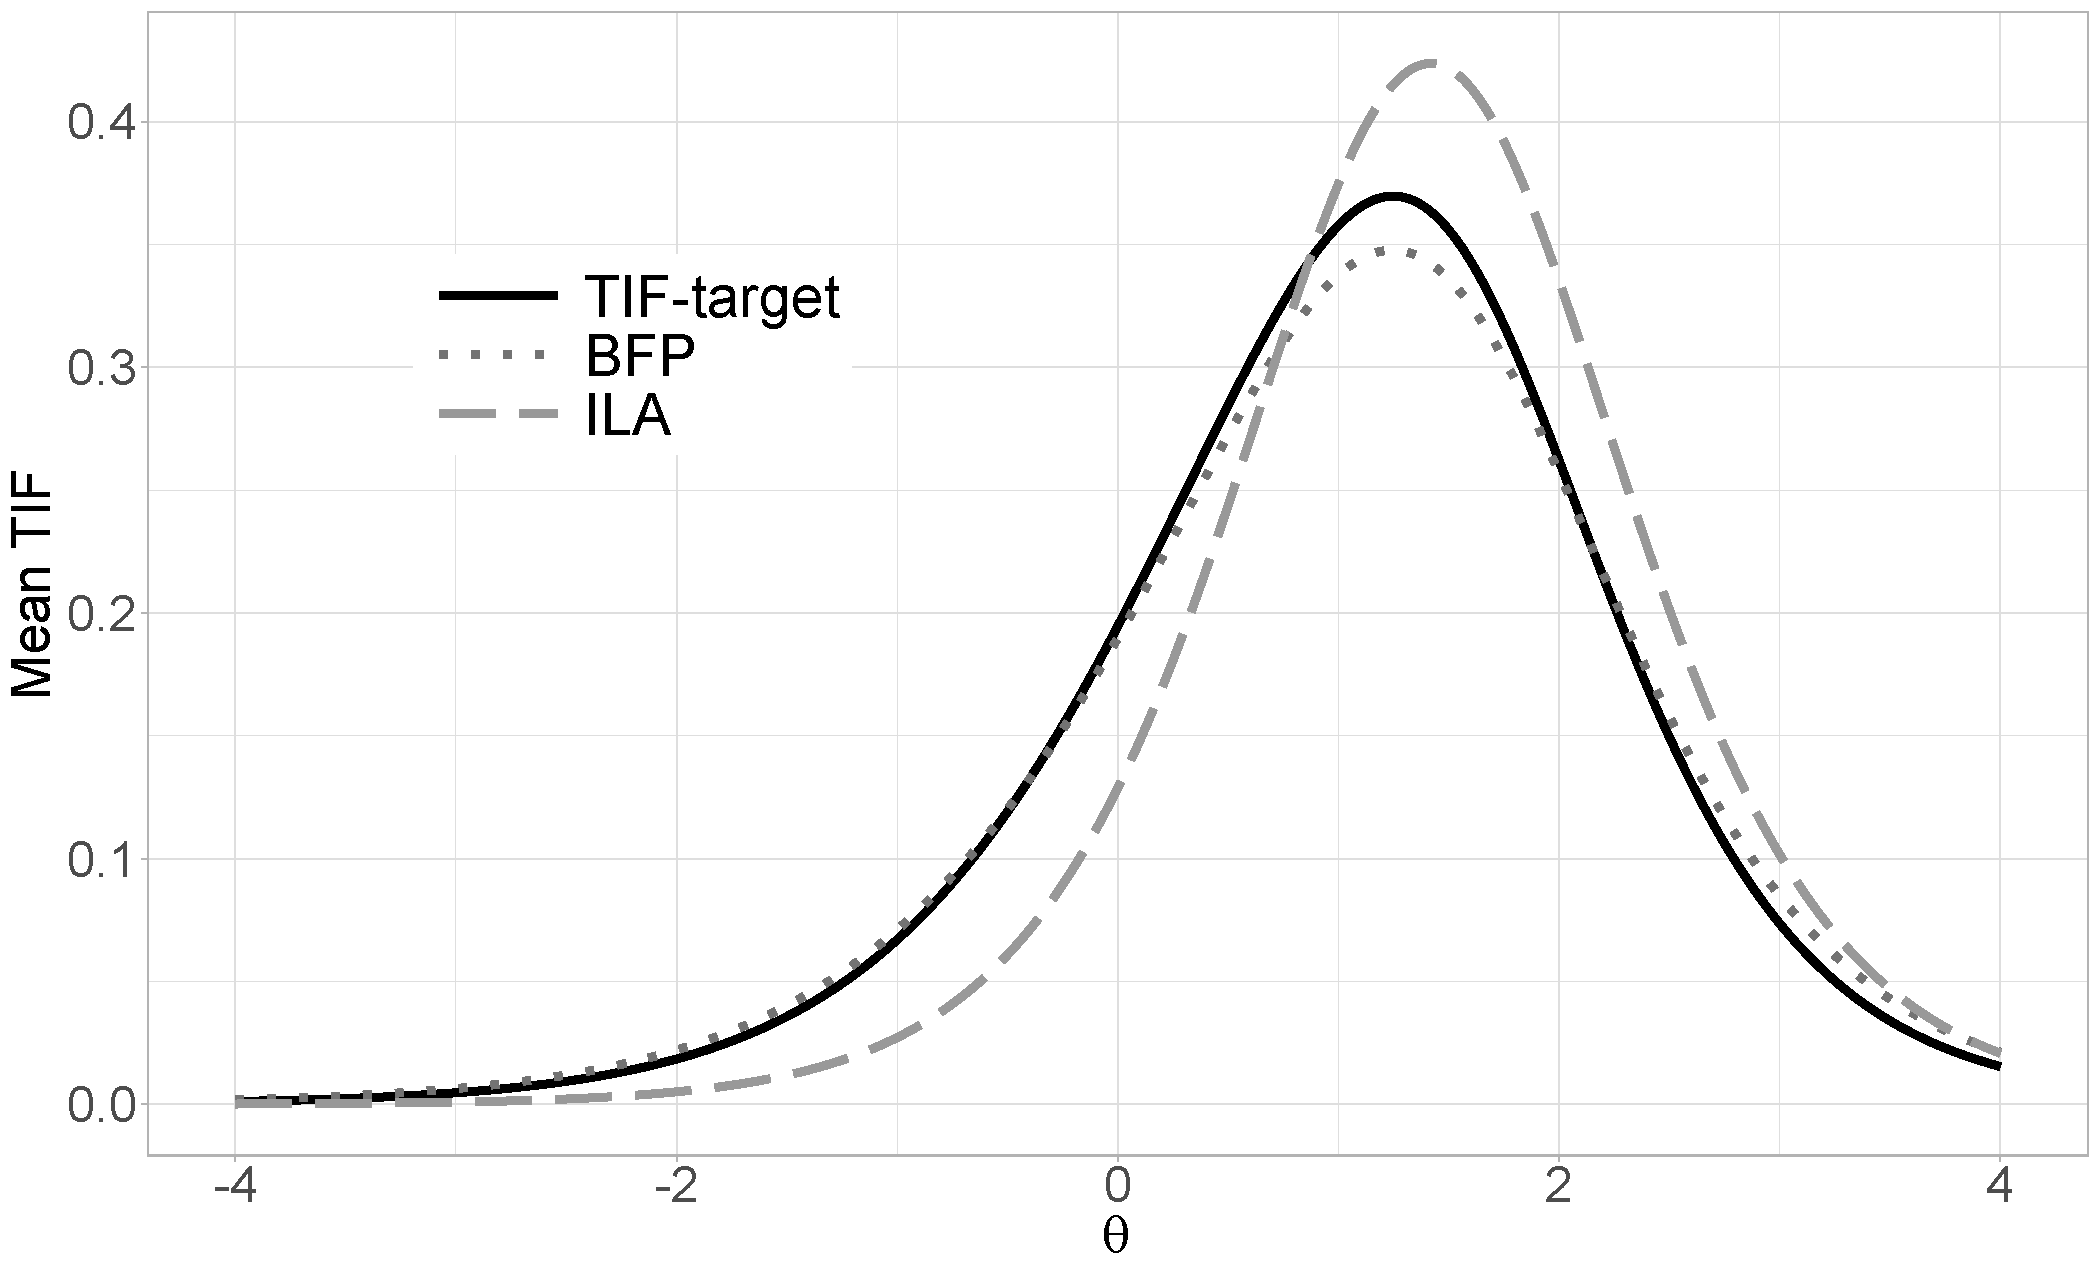
\includegraphics[width=.80\linewidth]{img/lessFar.pdf}	

		
	\end{column}
	\end{columns}
	

\end{frame}

\subsection{Conclusions}

\begin{frame}
	
	\begin{exampleblock}{\color{myGreen}\textbf{Pros of ILA}}
		
			\begin{itemize}
			\item It selects items that are able to recreate the desired characteristics of a test (usually)
			\item It is computationally ``Light'' 
		\end{itemize}
		
	\end{exampleblock}
	
	\begin{alertblock}{\color{unipd}Cons of ILA}
		
		\begin{itemize}
			\item It grounds its selection on a single $\theta_{target}$ at a time $\rightarrow$ it might select items minimizing the distance on that target but that are not very useful for the test 
			\item It only forwardly searches an item $\rightarrow$ once it is in, it can't get out
			\item It does not account for the discrimination parameters of the items
		\end{itemize}
	\end{alertblock}

\end{frame}


\end{document}
